\chapter{Операторные методы в квантовой механике. Метод вторичного квантования}

Общая идея этой главы состоит в получении результатов без перехода к какому-либо конкретному представлению. В результате получим метод, допускающий глубокие обобщения и являющийся основой {\em метода вторичного квантования}, нашедшего широкое применение в квантовой теории поля и физике конденсированного состояния.

\section{Операторы уничтожения и рождения в теории линейного гармонического осциллятора}

Собственные векторы $\ket{n}$ гамильтониана линейного гармонического осциллятора\footnote{<<Линейность>> осциллятора понимается в приближении одномерных малых колебаний вблизи положения равновесия} (ГО), отвечающие собственным значениям $E_n$, являются решениями уравнения

\begin{equation}
\label{eq:7_1_1}
\underbrace { \brc{ \frac{\op{p_x}^2}{2m} + \frac{m\omega^2 \op{x}^2}{2} } }_{\text{гамильтониан ГО}} \ket{n} = E_n \ket{n}
\end{equation}%
%
Здесь $m$ -- масса осциллятора, $\omega$ -- частота его колебаний. Введём операторы безразмерной координаты $\op{\xi}$ и безразмерного импульса $\op{p}_{\xi}$:

$$
\begin{gathered}
\op{\xi} = \frac{\op{x}}{a_0} = \sqrt{\frac{m\omega}{\hbar}} \op{x} \\
\op{p}_{\xi} = \frac{\op{p_x}}{p_0} = \frac{1}{\sqrt{m\hbar \omega}} \op{p_x}
\end{gathered}
$$%
%
где
$$
\begin{gathered}
a_0 = \sqrt{\frac{\hbar}{m\omega}}~\text{ -- {\em амплитуда нулевых колебаний}\footnotemark~ГО}\\
p_0 = \hbar/a_0 = \sqrt{m\hbar \omega}~\text{ -- отвечающией ей импульс.}
\end{gathered}
$$
\footnotetext{Происхождение этого названия будет понятно, когда найдём спектр.}

Обезразмерим уравнение \eqref{eq:7_1_1}, поделив его обе части на $\hbar \omega$:

$$
\underbrace{ \frac{1}{2} \brc{ \op{p_\xi}^2 + \op{\xi}^2} }_{\mathclap{\text{безразмерный гамильтониан}}} \ket{n} \equiv \op{h} \ket{n} = \epsilon_n \ket{n}
$$%
%
где $\epsilon_n = E_n/(\hbar \omega)$ -- безразмерная энергия. При этом операторы $\op{\xi}$ и $\op{p}_{\xi}$ удовлетворят коммутационному соотношению

\begin{equation}
\label{eq:7_1_2}
\brs{\op{\xi}, \op{p}_\xi} = \frac{1}{\hbar} \brs{\op{x}, \op{p}_x} = i
\end{equation}

Введём эрмитово сопряжённые (но не эрмитовы!) операторы $\ann$ и $\cre$, такие, что
$$
\left\{
\begin{aligned}
\ann \equiv \frac{\op{\xi} + i\op{p_\xi}}{\sqrt{2}} \\
\cre \equiv \frac{\op{\xi} - i\op{p}_\xi}{\sqrt{2}}
\end{aligned}
\right. ~~~ \Rightarrow ~~~ \left\{
\begin{aligned}
\op{\xi} = \frac{\ann + \cre}{\sqrt{2}} \\
\op{p}_\xi = \frac{\ann - \cre}{\sqrt{2}} \\
\end{aligned} \right.
$$%
%
Перепишем безразмерный гамильтониан $\op{h}$ через $\ann$ и $\cre$:
$$
\begin{gathered}
\cre\ann = \frac{1}{2} (\op{\xi} - i\op{p_\xi})(\op{\xi} + i\op{p_\xi}) = \left. \frac{1}{2}(\op{\xi}^2 + \op{p_\xi}^2 + i \brs{\op{\xi}, \op{p_\xi}}) \right|_{\text{\eqref{eq:7_1_2}}} =\\= \frac{1}{2} (\op{\xi}^2 + \op{p_\xi}^2 - 1) \equiv \op{h} - \frac{1}{2}
\\
\boxed{
  \op{h} = \cre\ann + \frac{1}{2}
}
\end{gathered}
$$%
%
В итоге уравнение \eqref{eq:7_1_1} на собственные векторы и собственные значения гамильтониана линейного ГО принимает вид
\begin{equation}
\label{eq:7_1_3}
\op{h} \ket{n} = \epsilon_n \ket{n}
\end{equation}

\section{Энергетрический спектр линейного гармонического осциллятора.}

Вычислим коммутатор $\ann$ и $\cre$:
$$
\begin{gathered}
\brs{\ann, \cre} = \frac{1}{2} \brs{ \op{\xi} + i\op{p_\xi},  \xi - i\op{p_\xi}} =\\= \frac{1}{2} \brc{ i\brs{\op{p_\xi}, \op{\xi}} - i \brs{\op{\xi}, \op{p_\xi}} } = -\frac{2i}{2} \underbrace{ \brs{\op{\xi}, \op{p_\xi}}}_{= i} = 1
\end{gathered}
$$
\begin{equation}
\label{eq:7_2_1}
\brs{\ann, \cre} = 1
\end{equation}%
%
Используя тождество $[\op{A}, \op{B}\op{C}] = [\op{A}, \op{B}] \op{C} + \op{B} [\op{A}, \op{C}]$ из \cref{ex:1_1_6}, получим:
\begin{equation}
\label{eq:7_2_2}
\brs{\cre, \op{h}} = \brs{\cre, \cre\ann} = \underbrace{\brs{\cre, \cre}}_{= 0} \ann + \cre \underbrace{\brs{\cre, \ann}}_{= -1} = - \cre
\end{equation}%
%
\begin{equation}
\label{eq:7_2_3}
\brs{\ann, \op{h}} = \brs{\ann, \cre\ann} = \underbrace{\brs{\ann, \cre}}_{= 1} \ann + \cre \underbrace{\brs{\ann, \ann}}_{= 0} = \ann
\end{equation}

Действуя на обезразмеренное уравнение \eqref{eq:7_1_3} слева оператором $\cre$, получаем
$$
\cre \op{h} \ket{n} = \epsilon_n \cre \ket{n}
$$%
%
или, с учётом \eqref{eq:7_2_2}:
\begin{equation}
\label{eq:7_2_4}
\op{h} \brc{\cre \ket{n}} = (\epsilon_n + 1)(\cre \ket{n})
\end{equation}%
%
Итак, если $\ket{n}$ -- собственный вектор гамильтониана линейного ГО, соответствующий собственному значению $\epsilon_n$, то $(\cre \ket{n})$ -- его собственный вектор, отвечающий собственному значению $(\epsilon_n + 1)$. Можно построить согласованные решения уравнений \eqref{eq:7_1_3} и \eqref{eq:7_2_4}, если принять следующие равенства

\begin{equation}
\label{eq:7_2_5}
\begin{gathered}
\epsilon_{n+1} \equiv \epsilon_n + 1 \\
\cre \ket{n} \equiv c_n \ket{n+1}
\end{gathered}
\end{equation}%
%
т.е. оператора $\cre$ увеличивает на единицу число квантов, поэтому он называется {\em оператором рождения} кванта колебаний. Коэффициент $c_n$ определяется из условия нормировки собственных векторов $\op{h}$:

\begin{equation}
\label{eq:7_2_6}
\begin{split}
\abs{c_n}^2 = \bk{\cre n}{\cre n} = \left. \bfk{n}{\ann\cre}{n} \right|_{\text{\eqref{eq:7_2_1}}} = \bfk{n}{\cre\ann + 1}{n} =\\= \bfkh{n}{\op{h} + \frac{1}{2}}{n} = \epsilon_n + \frac{1}{2}
\end{split}
\end{equation}

Аналогичным образом, действуя на \eqref{eq:7_1_3} слева оператором $\ann$, получаем
$$
\ann\op{h} \ket{n} = \epsilon_n \ann \ket{n}
$$%
%
или, с учётом \eqref{eq:7_2_3}:
\begin{equation}
\label{eq:7_2_7}
\op{h}(\ann\ket{n}) = (\epsilon_n - 1)(\ann \ket{n})
\end{equation}%
%
Если $\ket{n}$ -- собственный вектор гамильтониана линейного ГО, соответствующий собственному значению $\epsilon_n$, то $(\ann \ket{n})$ -- его собственный вектор, отвечающий собственному значению $(\epsilon_n - 1)$. Можно построить согласованные решения уравнений \eqref{eq:7_1_3} и \eqref{eq:7_2_7}, если принять следующие равенства

\begin{equation}
\label{eq:7_2_8}
\begin{gathered}
\epsilon_{n-1} \equiv \epsilon_n - 1 \\
\ann \ket{n} = c_{n}' \ket{n-1}
\end{gathered}
\end{equation}%
%
т.е. оператор $\ann$ уменьшает на единицу число квантов, поэтому он называется {\em оператором уничтожения} кванта колебаний. Коэффициент $c_n$ опять определяется из условия нормировки собственных векторов $\op{h}$:

\begin{equation}
\label{eq:7_2_9}
	\abs{c_n'}^2 = \bk{\ann n}{\ann n} = \bfk{n}{\cre\ann}{n} = \bfkh{n}{\op{h} - \frac{1}{2}}{n} = \epsilon_n - \frac{1}{2}
\end{equation}%
%
Поскольку $\abs{c_n'}^2 \geqslant 0$, то $\epsilon \geqslant 1/2$. Таким образом, среди собственных значений $\op{h}$ существует минимальное значение $\epsilon_0 = 1/2$. Ему отвечает собственный вектор $\ket{0}$, такой что (см.~\eqref{eq:7_2_8} и \eqref{eq:7_2_9})
$$
	\ann \ket{0} = 0
$$

Совокупность собственных значений $\op{h}$, согласно \eqref{eq:7_2_5} и \eqref{eq:7_2_8}, описывается формулой

\begin{equation}
\label{eq:7_2_10}
\epsilon_n = n + \frac{1}{2},~~ n = 0,1,2...
\end{equation}%
%
Следовательно, спектр линейного ГО имеет вид:
$$
\boxed {
	E_n = \hbar \omega \brc{n + \frac{1}{2}},~~ n = 0,1,2...
}
$$%
%
Характерной особенностью спектра линейного ГО является его {\em эквидистантность}: расстояние между двумя любыми соседними энергетическими уровнями равно $\hbar \omega$ (см.~\autoref{fig:7_1}).

\begin{figure}[h]
\centering
\begin{tikzpicture}[domain=-3.5:3.5]
   \draw[->] (-2.5,0) -- (2.5,0) node[right] {$x$};
  \draw[->] (0,-0.1) -- (0,4) node[above] {$U(x)$};
	\draw [domain=-2.0:2.0, samples=100] plot (\x, {\x*\x});
	\draw[dashed] (0.71,0.5) -- (0.71,0) node[below] {$a_0$};
	\draw[-] (-0.71,0.5) -- (0.71,0.5) node[right] {$n=0$};
	\draw[-] (-1.22,1.5) -- (1.22,1.5) node[right] {$n=1$};
	\draw[-] (-1.58,2.5) -- (1.58,2.5) node[right] {$n=2$};
	\draw[<->, thick] (0,2.5) -- (0,3.5);
	\node[right] at (0, 3) {$\hbar \omega$};
	\draw[-] (-1.87,3.5) -- (1.87,3.5) node[right] {$n=3$};
  \draw[dashed] (-2, 0.5) -- (-0.71, 0.5);
  \node[below] at (0, 0) {$0$};  
  \draw[<->] (-1.9, 0) -- (-1.9, 0.5) node[left] {$\dfrac{\hbar \omega}{2}$};
  \end{tikzpicture}
\caption{Спектр гармонического осциллятора.} \label{fig:7_1}
\end{figure}

При $n = 0$:
$$
\frac{\hbar \omega}{2} = \frac{m\omega^2}{2} a_0^2  ~~\to~~
\boxed{
  a_0 = \sqrt{\frac{\hbar}{m\omega}}
}
$$
-- амплитуда нулевых колебаний ГО.

Если коэффициенты $c_n$ и $c_n'$ выбрать действительными, то из соотношений \eqref{eq:7_2_6}, \eqref{eq:7_2_9} и \eqref{eq:7_2_10} вместо \eqref{eq:7_2_5} и \eqref{eq:7_2_8} имеем:
\begin{equation}
\label{eq:7_2_5_add}
\boxed {
	\cre\ket{n} = \sqrt{n+1}\ket{n+1}
}
\tag{\ref{eq:7_2_5}$'$}
\end{equation}%
% TODO: объединить в одно окружение
\begin{equation}
\label{eq:7_2_8_add}
\boxed {
	\ann\ket{n} = \sqrt{n}\ket{n-1}
}
\tag{\ref{eq:7_2_8}$'$}
\end{equation}%
%
соответственно. Поэтому операторы $\ann$ и $\cre$ ещё называют {\em понижающим} и {\em повышающим} соответственно.

\section{Построение собственных функций осциллятора в координатном представлении с помощью операторов рождения и уничтожения. Связь $n$-го состояния осциллятора с основным.}

Уравнение, определяющее вектор основного состояния линейного ГО $\ket{0} \equiv \ket{\psi_0}$, т.е. состояния с минимальной энергией $\epsilon_0$, может быть записано как
$$
\ann \ket{0} = 0 ~~~\text{или}~~~ \frac{1}{\sqrt{2}}(\op{\xi} + i\op{p_\xi}) \ket{\psi_0} = 0
$$%
%
В координатном $\xi$-представлении оно принимает вид
$$
\brc{\xi + \D{}{\xi}} \psi_0(\xi) = 0
$$%
%
Решая его, находим волновую функцию основного состояния линейного ГО в $\xi$-представлении, нормированную на единицу
$$
\boxed {
	\psi_0(\xi) = \frac{1}{\pi^{1/4}} e^{-\xi^2/2}
}
$$

Заметим теперь, что вектор $n$-го состояния линейного ГО $\ket{n} \equiv \ket{\psi_n}$ связан с вектором основного состояния соотношениями:

$$
\begin{gathered}
\cre \ket{0} = \sqrt{1} \ket{1} ~~~\to~~~ \ket{1} = \frac{1}{\sqrt{1}} \cre \ket{0} \\
\cre \ket{1} = \sqrt{2} \ket{2} ~~~\to~~~ \ket{2} = \frac{1}{\sqrt{2}} \cre \ket{1} = \frac{1}{\sqrt{2 \cdot 1}} (\cre)^2 \ket{0} \\
\cre \ket{2} = \sqrt{3} \ket{3} ~~~\to~~~ \ket{3} = \frac{1}{\sqrt{3}} \cre \ket{3} = \frac{1}{\sqrt{3 \cdot 2 \cdot 1}} (\cre)^3 \ket{0} \\
...\\
\boxed {
	\ket{\psi_n} \equiv \ket{n} = \sqrt{\frac{1}{n!}}(\cre)^n \ket{0}
}
\end{gathered}
$$%
%
Следовательно, в $\xi$-представлении для волновой функции $n$-го состояния линейного ГО получаем
$$
\psi_n(\xi) = \sqrt{\frac{1}{2^n \cdot n! \cdot \sqrt{\pi}}} \brc{\xi - \D{}{\xi}}^n e^{-\xi^2/2}
$$%
%
Эта волновая функция следующим образом выражается через $n$-й полином Эрмита:
$$
\boxed {
	\psi_n(\xi) = \sqrt{\frac{1}{2^n \cdot n! \cdot \sqrt{\pi}}} H_n(\xi) e^{-\xi^2/2}
}
$$
где $H_n(\xi) = e^{\xi^2/2} \brc{\xi - \D{}{\xi}}^n e^{-\xi^2/2} $

$$
H_0(\xi) = 1,~~ H_1(\xi) = 2\xi,~~ H_2(\xi) = 4\xi^2 - 2
$$%
%
Полином Эрмита $n$-й степени $H_n(\xi)$ имеет $n$ действительных корней, поэтому число нулей волновой функции ГО $\psi_n(x)$ равно $n$ (см.~\autoref{fig:7_2}). Это частный случай {\em осцилляторной теоремы} квантовой механики

\begin{thm}[Осцилляторная теорема]
Волновая функция $\psi_n(x)$, соответствующая собственному значению $E_n$, имеет при конечных $x$ ровно $n$ нулей.
\end{thm}

\begin{figure}[h]
  \centering
  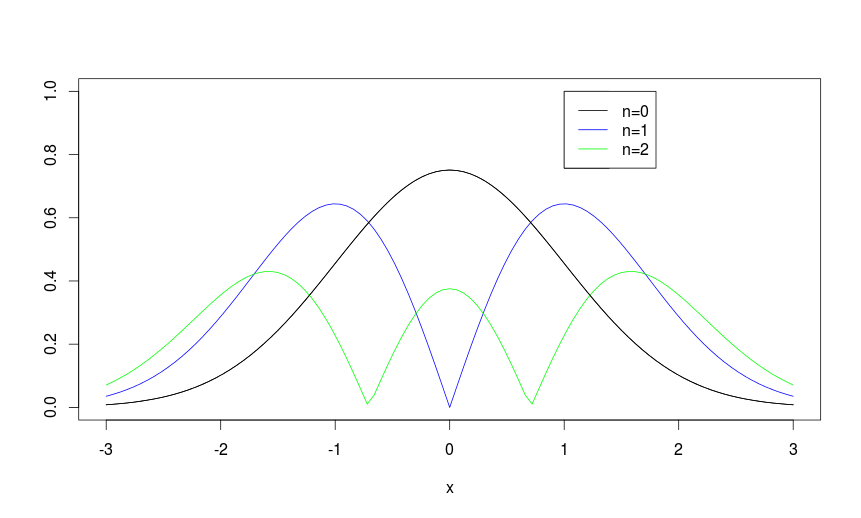
\includegraphics[scale=0.3]{figs/7_2}
  \caption{Модуль волновых функций гармонического осциллятора}
  \label{fig:7_2}
\end{figure}
